
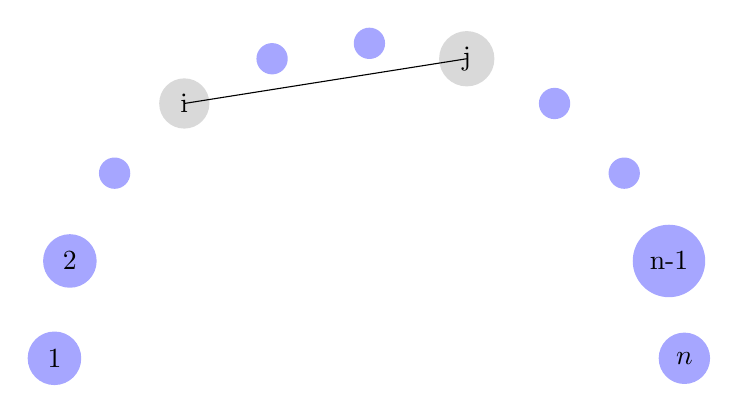
\begin{tikzpicture}[every node/.style={circle,inner sep=4pt}]

  \foreach \a in {0,1,2,...,10}{
  \draw (\a*360/20: 4cm) node[fill=blue!35]{};
  }
  
  \draw (10*360/20: 4cm) node[fill=blue!35]{1};
  \draw (9*360/20: 4cm) node[fill=blue!35]{2};
  \draw (1*360/20: 4cm) node[fill=blue!35]{n-1};
  \draw (0*360/20: 4cm) node[fill=blue!35]{$n$};
  
  \draw (7*360/20: 4cm) node[fill=black!15]{i};
  \draw (4*360/20: 4cm) node[fill=black!15]{j};
  
  \draw (7*360/20: 4cm) --(4*360/20: 4cm);
  
  \end{tikzpicture}